% =====================================================================
%  Figure panels for: A Semantically Inert Microkernel
%  Captions quote measured values; see validation/results/panel_stats.json
% =====================================================================

\begin{figure*}[!htbp]
    \centering
    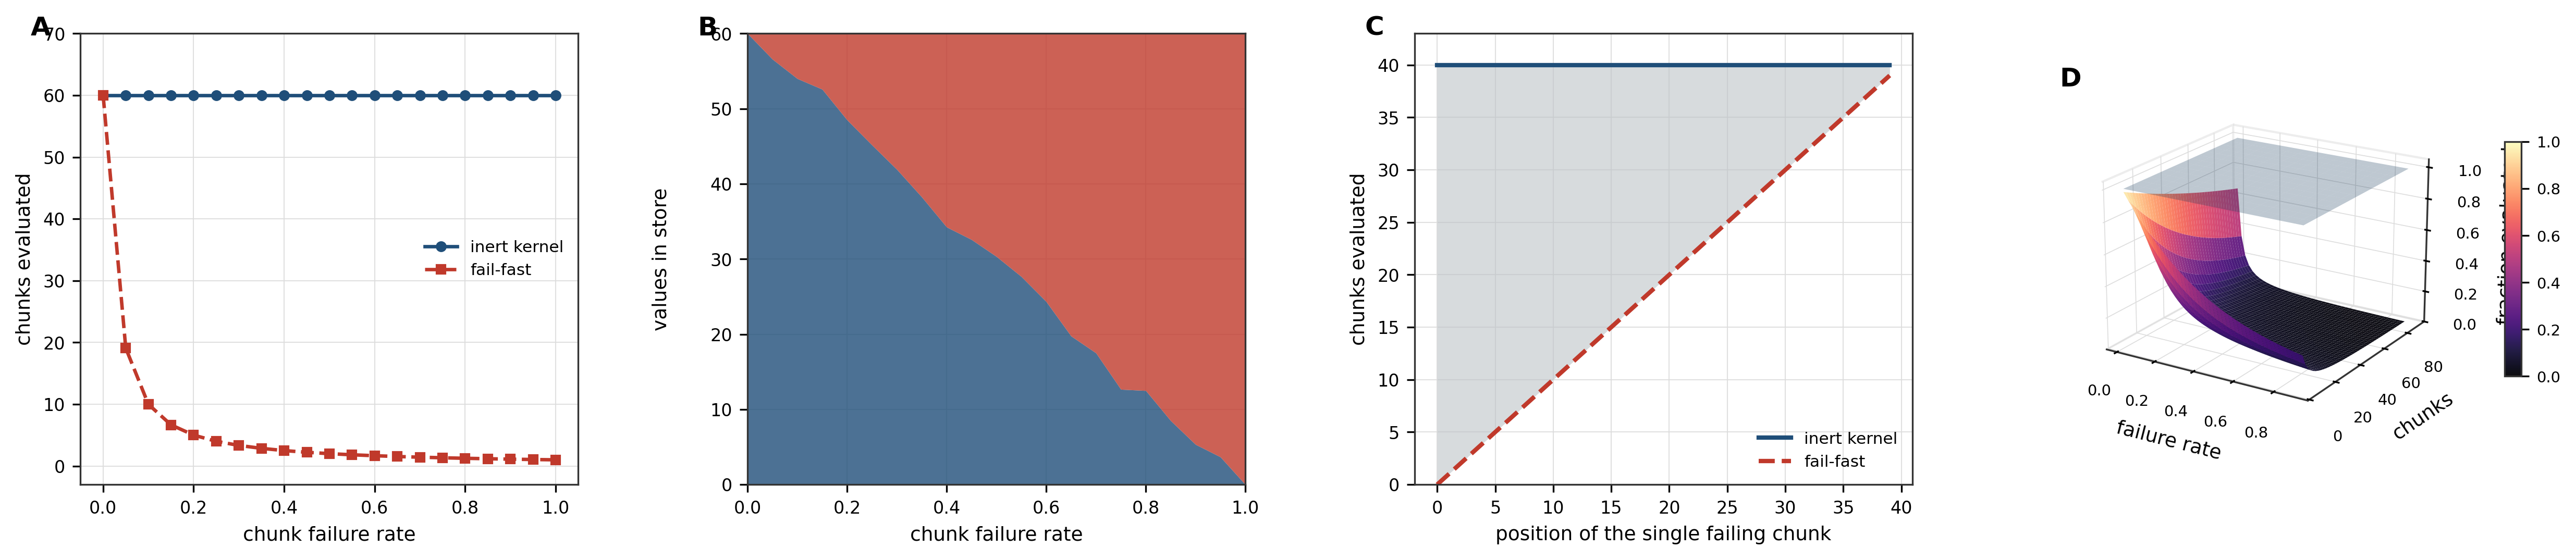
\includegraphics[width=\textwidth]{figures/panel_1_inertia.png}
    \caption{\textbf{Inertia: the quantity a fail-fast runtime destroys is evidence, and how much it destroys depends on an ordering that carries no meaning.}
    All quantities are measured by executing the kernel of \Cref{sec:kernel} rather than by simulating its behaviour; a chunk that raises produces an error value through the same path as any other value, so the counts below are of actual emissions. The fail-fast comparison is the exact expectation for a runtime halting at the first raising chunk, $\sum_{i<N}(1-p)^i$, not an approximation.
    (\textbf{A})~Chunks evaluated against per-chunk failure rate, for a node carrying $60$ chunks, $12$ repetitions at each of $21$ rates. The inert kernel evaluates all $60$ at every rate without exception, the flat upper line; the fail-fast comparison falls to $2.0$ at a failure rate of $0.5$ and to $1.0$ when every chunk raises. This is \Cref{cor:completion}: the kernel's execution sequence is not conditioned on emitted content, because by \Cref{thm:inertia} no kernel-computable quantity depends on that content.
    (\textbf{B})~Composition of the resulting value store, ordinary values below and error values above. The total is constant at $60$ across the whole range while the partition between the two shifts; at a failure rate of $0.5$ the store holds $29.7$ error values alongside $30.3$ ordinary ones, and all of them remain readable. Because $\emit$ adjoins rather than replaces (\Cref{cor:anomaly}), an anomaly is retained as data rather than consuming the run.
    (\textbf{C})~The decisive comparison: chunks evaluated when exactly \emph{one} chunk in a bag of $40$ raises, as a function of where that chunk sits in the bag. The inert kernel evaluates all $40$ regardless of position; the fail-fast count is the position itself, sweeping from $0$ to $39$. The shaded region between them is evidence destroyed, and its size is set entirely by an ordering within a chunk bag---which, the bag being a multiset, is not a meaningful property of the protocol. A single early anomaly can discard an arbitrary fraction of a run under fail-fast semantics and none of it here.
    (\textbf{D})~Expected fraction of a protocol evaluated, over failure rate and protocol size. The flat upper surface at unity is the inert kernel. The lower surface is fail-fast, and it falls away in both arguments: the larger the protocol, the greater the share lost to a fixed failure rate. The design cost is real and is stated in \Cref{rem:inertia-cost}---the kernel spends cycles on chunks a human reader would already have judged doomed---but the quantity traded away is compute, and the quantity retained is the record.}
    \label{fig:kpanel1}
\end{figure*}

\begin{figure*}[!htbp]
    \centering
    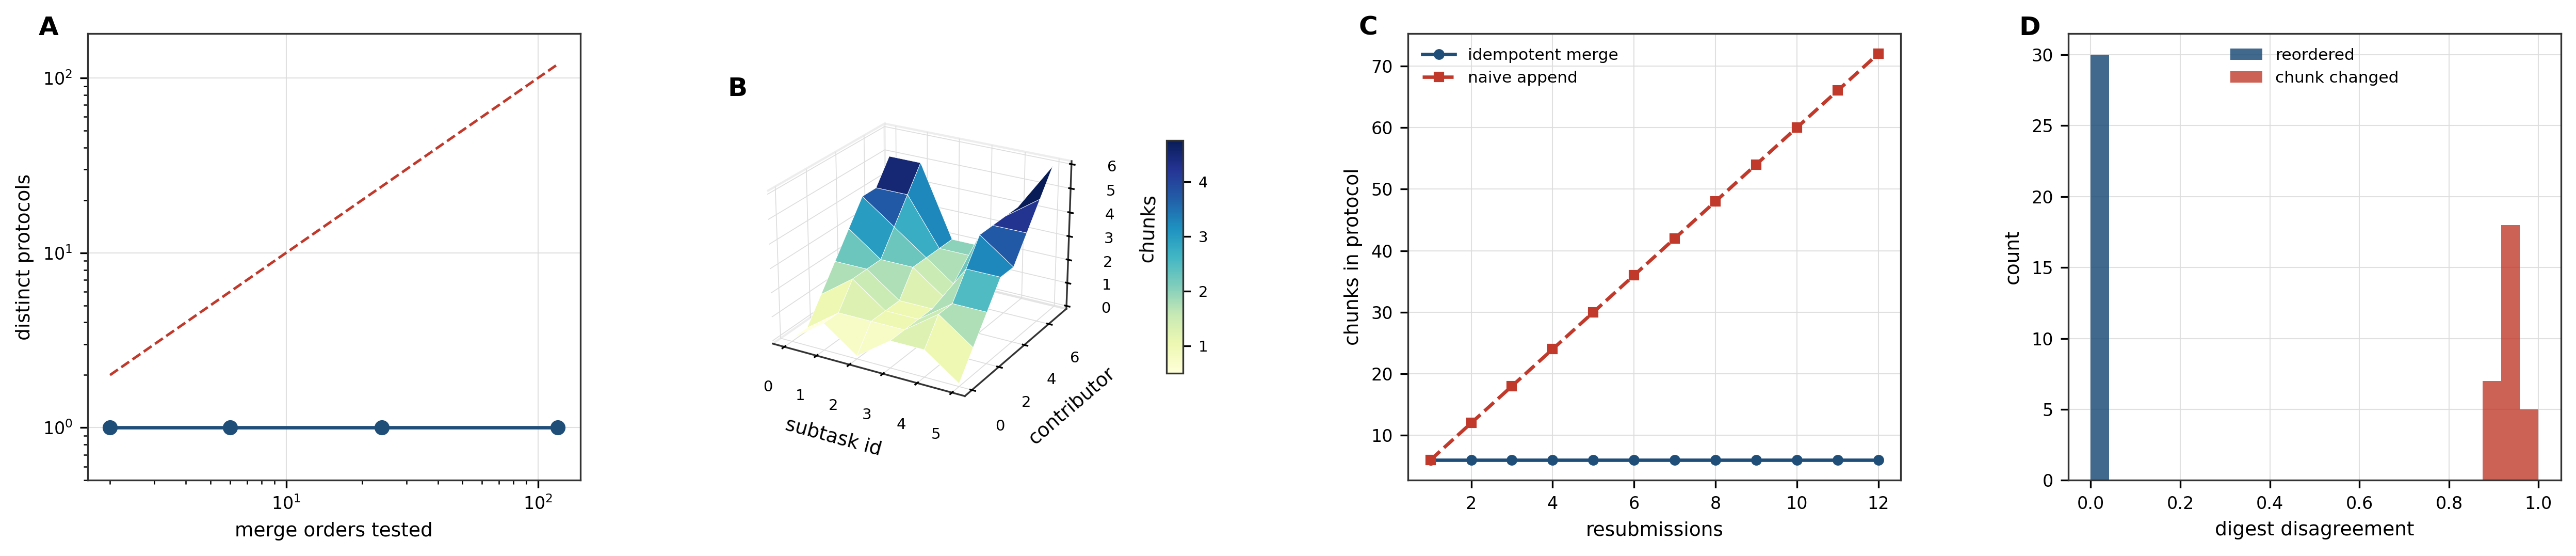
\includegraphics[width=\textwidth]{figures/panel_2_convergence.png}
    \caption{\textbf{Independently derived decompositions merge to one protocol, and the fingerprint separates the two things a reader needs to distinguish.}
    Contributions are sets of chunks keyed by subtask identity, with chunks identified by content, as \Cref{rem:identity} requires; every merge order is enumerated exhaustively rather than sampled, so the invariance below is exact over the space tested and not a statistical claim.
    (\textbf{A})~Distinct protocols obtained against the number of merge orders tested, for two to five contributors, $152$ orderings in total and up to $120$ for a single contributor set. The count is $1$ at every point, against the dashed line marking what would be obtained if order mattered. This is \Cref{thm:convergence-monoid}: merge is associative, commutative and idempotent, so the protocol is a function of the set of contributions and of nothing else about how they arrived.
    (\textbf{B})~Chunk accumulation on subtask identities as contributors arrive in sequence. Where two contributors independently reach the same identity, their chunks accumulate on a single node---the ridges---rather than producing parallel nodes. Convergence is what makes the surface rise rather than widen, and it depends on identities being derived from what a subtask \emph{is}, an obligation the kernel places on the layer above it and does not itself discharge.
    (\textbf{C})~Total chunks in the protocol against repeated resubmission of an identical contribution. Idempotent merge holds at $6$ chunks through twelve resubmissions; a naive append reaches $72$. The distinction matters operationally: a contributor that re-submits after a network retry must not thereby alter the protocol, and \Cref{thm:convergence-monoid} guarantees it does not.
    (\textbf{D})~Disagreement between protocol fingerprints, as the fraction of differing characters in the $64$-character digest. Reordering the contributions leaves every character identical (disagreement exactly $0.0$ in all $30$ trials); altering a single chunk changes $93.5$ per cent of characters on average, never fewer than $89.1$. The fingerprint is therefore stable under the transformations that do not change what can be computed and sensitive to those that do, which is what \Cref{thm:fingerprint} requires of it and what makes \Cref{cor:repro} operational.}
    \label{fig:kpanel2}
\end{figure*}

\begin{figure*}[!htbp]
    \centering
    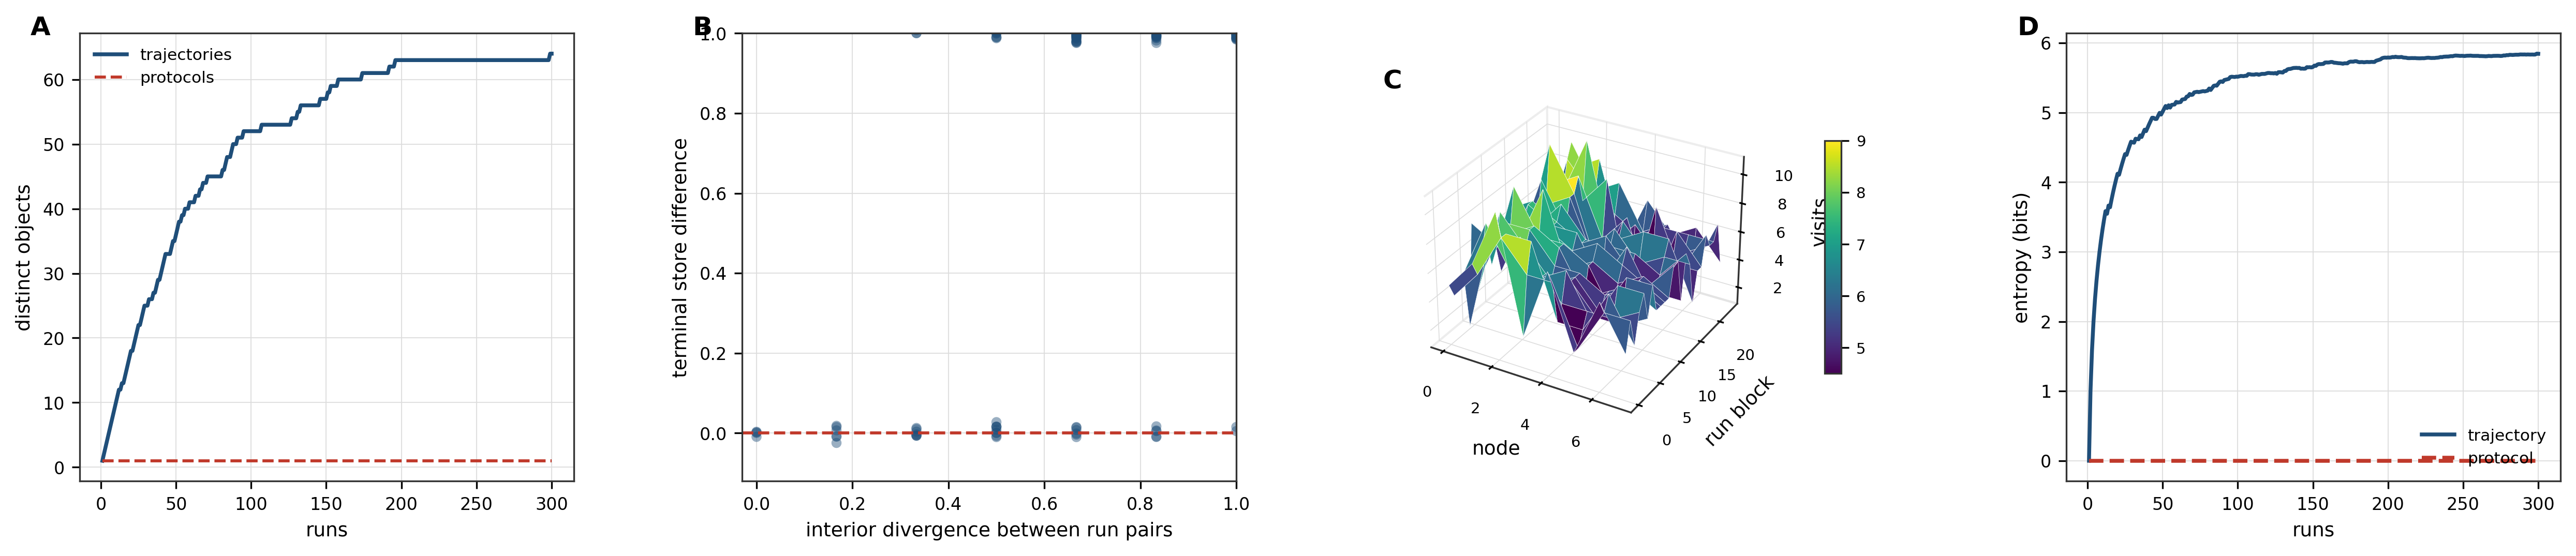
\includegraphics[width=\textwidth]{figures/panel_3_trajectory.png}
    \caption{\textbf{Protocol and trajectory are different objects, and the trajectory is recoverable from neither the protocol nor the result.}
    $300$ runs of a single fixed protocol whose probe chunk consults a varying external source, with the interior branching on the value read. The two charts on the left establish the two halves of the separation, and their conjunction is what restricts reproducibility claims.
    (\textbf{A})~Distinct protocols and distinct trajectories accumulated over the $300$ runs. The protocol count is $1$ throughout---every run has the identical node set and chunk bags, and the identical fingerprint---while the trajectory count rises to $64$ and is still rising slowly at the right edge. This is \Cref{thm:emergence}: the trajectory is not a function of the protocol, hence not computable in advance of the run and not storable as a schedule.
    (\textbf{B})~Interior divergence between pairs of runs that share a terminal store, against the difference observable at the terminus. The interiors differ by up to the full path length of $6$ while the terminal difference is identically zero for every pair. Three distinct functions of the store were probed---cardinality, sorted representation, and a cryptographic digest---and none separates any pair. This is \Cref{thm:opacity}, and with (A) it places the trajectory outside the closure of the two data a reader normally holds: what was asked, and what came back.
    (\textbf{C})~Node visitation counts across blocks of runs. The set of nodes visited is fixed by the protocol; the counts vary between blocks because the route through them does not. The surface is the same object as (A) resolved by node rather than by run.
    (\textbf{D})~Empirical entropy of the trajectory distribution against the number of runs, with the protocol entropy drawn for comparison. The trajectory accumulates $5.01$ bits by run $50$ and $5.84$ bits by run $300$; the protocol contributes exactly $0$ at every point. The gap is the information a system logging only protocol and terminal store would be unable to reconstruct even in principle, which is the argument of \Cref{rem:record-limits} for recording the read-to-emit relation explicitly.}
    \label{fig:kpanel3}
\end{figure*}

\begin{figure*}[!htbp]
    \centering
    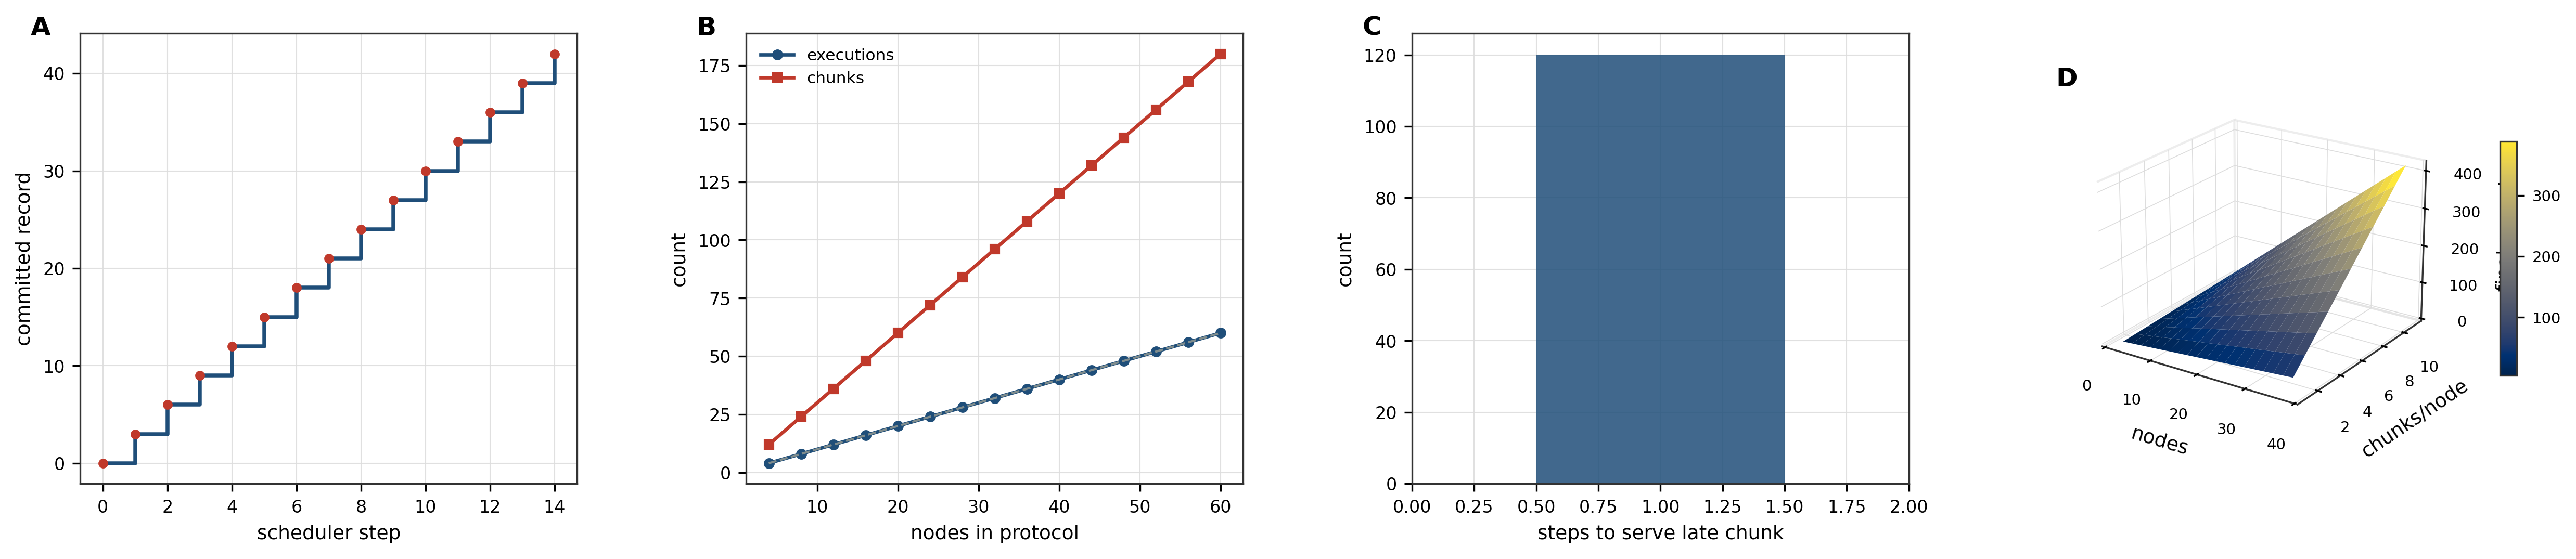
\includegraphics[width=\textwidth]{figures/panel_4_scheduler.png}
    \caption{\textbf{The committed record orders a run without a clock, and the scheduler is exact rather than merely adequate.}
    The scheduler selects uniformly at random from the ready set, which is a fair rule in the sense of \Cref{def:scheduler} but the least favourable such rule for the guarantees below; the counts are therefore not artefacts of a helpful selection order.
    (\textbf{A})~Committed record against scheduler step for a sweep over fourteen nodes carrying three chunks each. The record is a strictly increasing staircase, advancing by exactly three at each node visit and never decreasing. Because no operation in the vocabulary removes a value or decrements the count, two states with equal value stores and unequal records are distinct (\Cref{thm:monotone}): a recurring configuration is not a return, and the ordering is available without reference to wall-clock time (\Cref{cor:clock}).
    (\textbf{B})~Executions and committed chunks against protocol size. The execution count equals the node count exactly at every size tested, up to $60$ nodes, and the committed record equals the total chunk count, reaching $180$ at the largest protocol. Each node is therefore visited once and all its pending chunks are evaluated in that visit, which is the no-redundant-re-execution clause of \Cref{thm:scheduler}(i) measured rather than assumed.
    (\textbf{C})~Steps required to serve a chunk contributed \emph{after} a sweep has completed and every node has gone quiescent, over $120$ trials. Every late chunk was served in exactly one step and none was starved. The result is stronger than \Cref{thm:scheduler}(ii) requires---the theorem guarantees only eventual service---and it holds because a contribution makes its node ready again immediately, so the readiness rule needs no notion of priority or ageing.
    (\textbf{D})~Final committed record over protocol size and chunks per node. The surface is exactly the product of its two arguments, with no deviation at any grid point, confirming that the record counts committed evaluations and nothing else: no retries, no speculative execution, no bookkeeping steps enter it. This is what makes the record usable as a provenance ordinal.}
    \label{fig:kpanel4}
\end{figure*}
